\section{Logarithms}

\dfn{Logarithms}{
	\(a^x = y \therefore \log_ay=x\)
}
\begin{tabular}{cc}
	Exponential Fact & Logarithm Fact \\ \\
	\hline \\
	\(10^3 = 1000\) & \(\log_{10}1000 = 3\) \\ \\
	\(5^4 = 625\) & \(\log_5{625} = 4\) \\ \\
	\(36^{\frac{1}{2}} = 6\) & \(log_{36}6 = \frac{1}{2}\) \\ \\
	\(2^{-3} = \frac{1}{8}\) & \(log_2{\frac{1}{8}} = 3\)
\end{tabular}

\subsection{Log Laws}
\dfn{Log \& Index Laws}{
	\begin{tabular}{cc}
		Laws of Indices & Laws of Logs \\ \\
		\hline \\
		\(a^x * a^y = a^{x+y}\) & \(\log_ax + \log_ay = \log_amn\) \\ \\
		\(a^x \div a^y = a^{x-y}\) & \(\log_ax - \log_ay = \log_a\frac{x}{y}\) \\ \\
		\(\left( a^x \right) ^y = a^{xy}\) & \(\log_ax * \log_ay = \log_am^n\)
	\end{tabular}
}

\qs{\(\log_4\frac{x}{x-1} = \log_43 + log_42\)}{
	\begin{align*}
		\log_4\frac{x}{x-1} &= \log_46 \\
		\frac{x}{x-1} &= 6 \\
		x &= 6x - 6 \\
		\ldots
	\end{align*}
}
\qs{\(\log_74x = \log_7\frac{1}{x-6} + 1\)}{
	\begin{align*}
		\log_7\frac{4}{\frac{1}{x-6}} &= 1 \\
		\log_74x(x-6) &= 1 \\
		\log_74x^2-24x &= 1 \\
		4x^2-24x &= 7 \\
		\ldots
	\end{align*}
}
\qs{\(2^x=75\)}{
	\begin{align*}
		x &= \log_275 \\
		x &= 6.23
	\end{align*}
}
\qs{\(5^{2x} - 6\left( 5^x \right) = 0\)}{
	\begin{align*}
		\text{let } y &= 5^x \\
		y^2 - 6y - 7 &= 0 \\
		(y - 7)(y + 1) &= 0 \\
		\text{Logarithms always positive} \therefore y &= 7 \\
		5^x &= 7 \\
		x &= log_57 \\
		x &= 1.21 \\
	\end{align*}
}
\qs{\(3^{2x+1} = 2^{5x}\)}{
	\begin{align*}
		\log_e3^{2x+1} &= \log_e2^{5x} \\
		(2x+1)\log_e3 &= (5x)\log_e2 \\
		2(\log_e3)x + \log_e3 &= 5(log_e2)x \\
		\log_e3 &= 5(\log_e2)x - (2log_e3)x \\
		\log_e3 &= x(5log_e2 - 2loge_3) \\
		x &= \frac{log_e3}{5log_e2 - 2loge_3} \\
		x &= 0.866
	\end{align*}
}


\section{Exponentials}
\begin{plotter}
	\addplot [
		domain=-2:2,
		samples=100,
		color=black,
	]
	{2^x};
	\addlegendentry{\(2^x\)}
	\addplot [
		domain=-2:2,
		samples=100,
		color=black,
	]
	{2*2^x};
	\addlegendentry{\(2*2^x\)}
\end{plotter}

Graphs with anything to the power of \(x\) always have a y-intercept of 1, because anything to the power of 0 is equal to 1.

\subsection{Euler's Number - \(e\)}
\dfn{\(e\)}{
	\(e\) is defined as having the following characteristics:
	\begin{itemize}
		\ii \(y = e^x\), \(\differen = e^x\)
		\ii \(y = e^{kx}\), \(\differen = ke^{kx}\)
	\end{itemize}
}

\nt{\[ \log_ex \equiv \ln{x} \]}

\qs{\(y = Ae^{kx}\), and passes through \((0,6)\) and \(1,9\). Find \(A\) and \(k\)}{
	\begin{align*}
		6 &= Ae^0 \\
		A &= 6 \\ \\	
		9 &= 6e^k \\
		e^k &= \frac{9}{6} \\
		k &= \ln\frac{9}{6} \\
		k &= 0.41
	\end{align*}
}

\section{Modelling With Exponentials}
All Exponentials can be written with \(e\), which makes calculus much easier.

Given \(y = Ae^{kx}\), if \(k > 0\) we get exponential growth, and if \(k < 0\) then we get exponential decay.

When modelling with exponentials, \(A\) typically represents the initial population, and \(k\) the growth/decline factor.

\section{Logarithm Graphs}

As you might expect, logarithm graphs are just exponential graphs reflected in \(y=x\).

\begin{tikzpicture}
\begin{axis}[
		axis lines = center,
		ymin=-10,ymax=10,
		xlabel = \(x\),
		ylabel = \(f(x)\),
	]
	\addplot [
		domain=-5:5,
		samples=100,
		color=black,
	]
	{e^x};
	\addlegendentry{\(e^x\)}
	\addplot [
		domain=0:5,
		samples=250,
		color=blue,
	]
	{ln(x)};
	\addlegendentry{\(\ln{x}\)}
\end{axis}
\end{tikzpicture}


\section{Logs \& Non-Linear Data}
When given non-linear data, we can use logs to extrapolate from it and find an equation. Usually, we can take logs of the \(y\) equivalent and then plot \(x\) vs \(\log{y}\).
\qs{\(B = Ak^t\), where \(t\) represents days and \(B\) represents the population, find \(k\) and \(A\)}{
	\begin{tabular}{rl}
		Days & Population \\
		\hline
		\(1\) & \(24\) \\
		\(2\) & \(28\) \\
		\(3\) & \(36\) \\
		\(4\) & \(40\) \\
		\(5\) & \(50\) \\
	\end{tabular}

	\ex{Solving Graphically}{
		\begin{alignat*}{3}
			B &= A &*&& k^t\\ \\
			y &= xm &+&& c \\
			\log{B} &= t\log{k} &+&& A
		\end{alignat*}
	
		\begin{tabular}{llr}
			\(t\) & \(B\) &  \(\log{B}\) \\
			\hline
			\(1\) & \(24\) & \(1.38\) \\
			\(2\) & \(28\) & \(1.45\) \\
			\(3\) & \(36\) & \(1.56\) \\
			\(4\) & \(40\) & \(1.60\) \\
			\(5\) & \(50\) & \(1.70\) \\
		\end{tabular}
	
		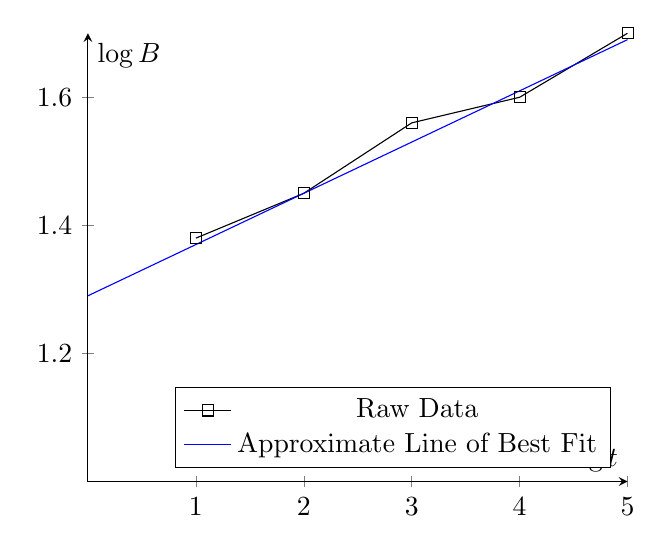
\begin{tikzpicture}
		\begin{axis}[
				axis lines = center,
				ymin=1,
				xlabel = \(\log{t}\),
				ylabel = \(\log{B}\),
				legend pos=south east,
			]

			\addplot [
				color=black,
				mark=square,
			]
			coordinates {
				(1,1.38)(2,1.45)(3,1.56)(4,1.6)(5,1.7)
			};
			\addlegendentry{Raw Data}
		
			\addplot [
				domain=0:5,
				samples=100,
				color=blue,
			]
			{0.08*x+1.29};
			\addlegendentry{Approximate Line of Best Fit}
		\end{axis}
		\end{tikzpicture}
	
		From the line of best fit, we can see that the y-intercept is \(1.29\) and using non-shown calculations, we can see that the gradient is \(0.08\)
		
		\begin{align*}
			1.3 &= \log{k} \\
			k &= 10^{1.3} \\
			k &= 19.95 \\ \\
			0.08 &= \log{A} \\
			A &= 10^{0.08} \\
			A &= 1.20
		\end{align*}
	
		\(k = 19.95\) and \(A = 1.20\)
	}
}